\documentclass[tikz,border=10pt]{standalone}
\usepackage{tikz}
\usetikzlibrary{matrix}

\tikzset{
  cell/.style={draw=black!70, line width=1.0pt, minimum width=4.8cm, minimum height=1.15cm, align=center, text width=4.4cm, fill=none},
  head/.style={cell, draw=blue!70!black, line width=1.2pt},
  left/.style={cell, draw=green!50!black, line width=1.2pt}
}

\begin{document}
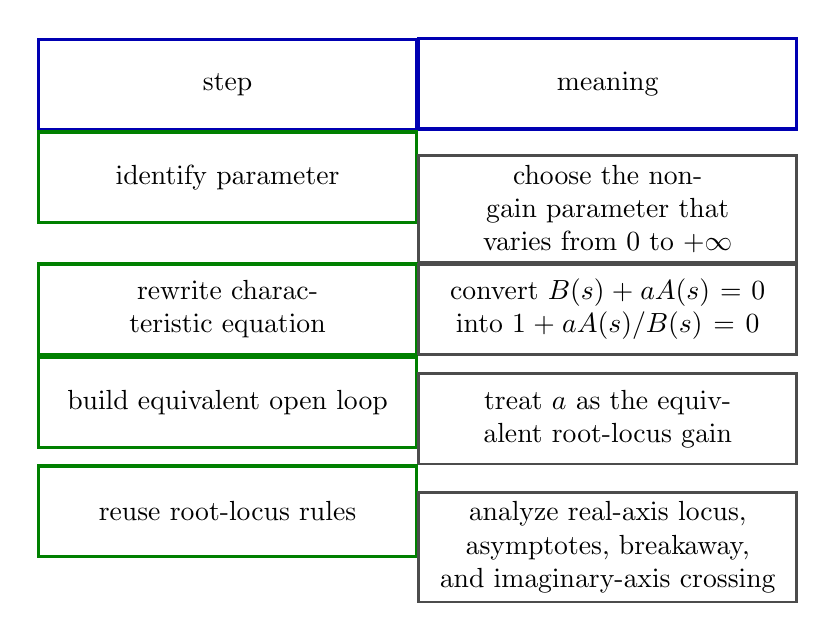
\begin{tikzpicture}
  \matrix[matrix of nodes, nodes in empty cells, row sep=-\pgflinewidth, column sep=-\pgflinewidth] {
    \node[head] {step}; &
    \node[head] {meaning}; \\
    \node[left] {identify parameter}; &
    \node[cell] {choose the non-gain parameter that varies from $0$ to $+\infty$}; \\
    \node[left] {rewrite characteristic equation}; &
    \node[cell] {convert $B(s)+aA(s)=0$ into $1+aA(s)/B(s)=0$}; \\
    \node[left] {build equivalent open loop}; &
    \node[cell] {treat $a$ as the equivalent root-locus gain}; \\
    \node[left] {reuse root-locus rules}; &
    \node[cell] {analyze real-axis locus, asymptotes, breakaway, and imaginary-axis crossing}; \\
  };
\end{tikzpicture}
\end{document}
